\chapter{Interfaces for Hardware Design}
One of the goals of \chai \ is to formally verify hardware designs
%<<<<<<< mv2rm.tex
%at the Register Transfer Logic (RTL) level. {\chai } has a Binary
%=======
at the Register Transfer Logic (RTL) level. {\chai} has a Binary
%>>>>>>> 1.19
Decision Diagram (BDD) based formal verification engine and has
algorithms to compose and verify designs. A developer can use
these algorithms to formally verify existing hardware designs.
Tools for converting existing component based hardware designs to
the \chai \ environment are required to be able to provide such a
comprehensive test bed for component-based design verification
algorithms and methodologies. This chapter describes the
conversion of hardware designs coded in Verilog, Esterel or VHDL
to Interface Modules, as summarized in Figure \ref{fig:hdl2intf}.

\begin{figure}[htbp]
\centering
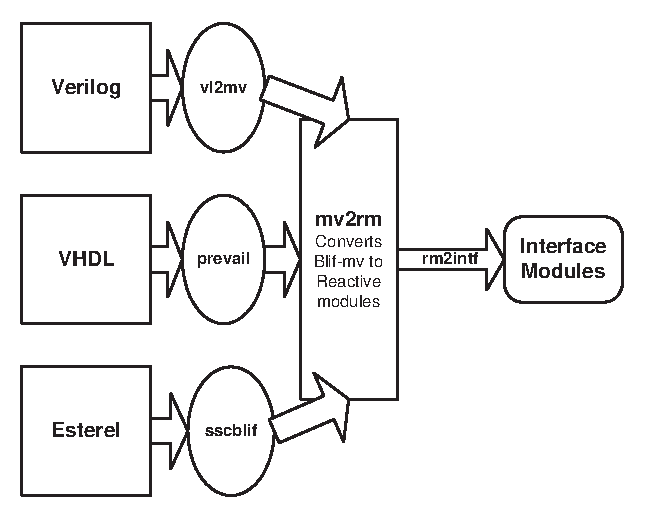
\includegraphics[width=4in]{figs/hdl2intf}
\caption{Converting Hardware Description Languages to Interfaces}
\label{fig:hdl2intf}
\end{figure}

\section{HDL to BLIF-MV}
Verilog to \mv \ conversion is possible by the tool vl2mv
\cite{vl2mv}. VHDL to \mv \ conversion can be achieved by the tool
prevail \cite{PREVAIL} while Esterel has a back-end SSCBlif
\cite{sscblif} to output code in \mv \ format. Thus, \mv \ is a
rich intermediate format.

\section{{\mv }}
\mv \ is an acronym for Berkeley Logic Interchange Format ---
Multivariate. It is successor of BLIF, and it primarily adds
non-determinism. The \mv \ format is designed to represent
non-deterministic sequential systems in hierarchical fashion. A
system can be composed of interacting sequential systems, each of
which can be again described as a collection of communicating
sequential systems. In {\mv }, there is an implicit assumption
that the whole system is clocked by a single global clock,
although the clock is never declared in {\mv }.

We implemented a tool to convert a \mv \ representation of a
design to reactive modules. The next two sections describe the tool
\mvrm \ and the translation process.

\subsection{MV2RM}
\begin{figure}[htbp]
\resizebox{3in}{!}
{\includegraphics[0,0][3in,3in]{figs/car}}
\caption{Pedestrian Crossing} \label{fig:piclights}
\end{figure}

Figure \ref{fig:piclights} illustrates a simple daily life
scenario of a pedestrian crossing. Here a simple traffic light
%<<<<<<< mv2rm.tex
%controller manages both the car traffic lights and the pedestrian
%=======
controller manages the car traffic lights and the pedestrian
%>>>>>>> 1.19
lights. Figure \ref{fig:pedlight} presents the example encoded in
{\mv}. When the \emph{CarSignal} is asserted and Mr. Bean pushes
\emph{Button} to cross the street then the \emph{ControlLogic}
de-asserts the \emph{CarSignal} at next clock-tick. When
\emph{CarSignal} is de-asserted the \emph{PedestrianSignal} gets
asserted. Finally, now Mr. Bean is able to cross the road!

The left column in Figure \ref{fig:pedlight} is the {\mv } model
\cite{b2m} and the right column is translation to {\rm } done by
{\mvrm }.

\begin{figure}
\centering
\includegraphics[1,0][7in,8in]{figs/modelLights}
%\input{egs/lights.mv}
%\hspace{4em}
%\input{egs/lights.rm}
\caption{Pedestrian Light Controller in BLIF-MV and {\rm}}
\label{fig:pedlight}
\end{figure}

Figure \ref{fig:mv2rmarch} shows the architecture of \mvrm . The
file {\tt lights.mv} is fed to the lexer of {\mvrm }. The
translation is two-pass. {\mvrm } is implemented in function
language OCAML \cite{ocaml}.

In pass one the \textbf{sub-circuit analyzer} parses the input
models {\mv } to analyze the parameters of the subcircuits used to
make an appropriate hide variable list when the model is converted
in to a {\rm }.

In pass two the \textbf{parser} goes through all the \mv \
constructs to make an abstract syntax tree. The validation of
input is done in this phase. At the end of the pass the code
generator runs over the abstract syntax tree to emit \rm \ code.

\begin{figure}[htbp]
\centering \resizebox{4in}{!}{
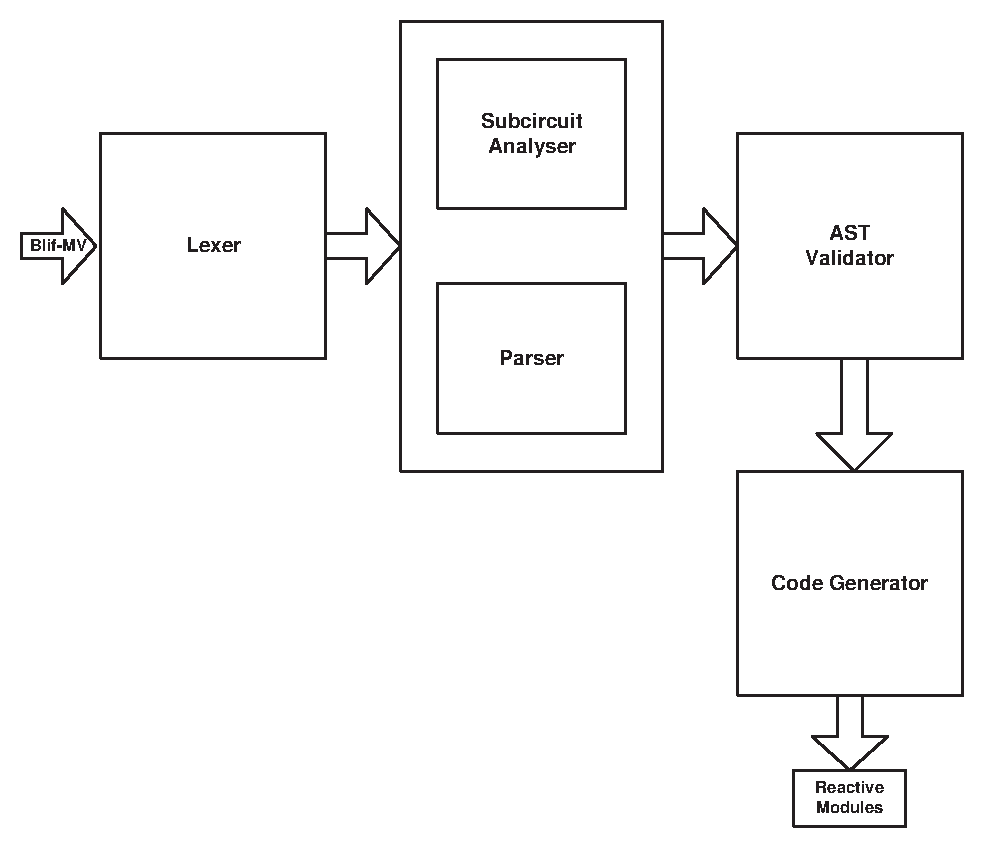
\includegraphics[width=4in,bb= 20 20 600 400]{figs/mv2rmarch}}
\caption{Architecture of {\mvrm} } \label{fig:mv2rmarch}
\end{figure}


\section{Translating {\mv } to {\rm }}
In this section we describe the translation logic used by
{\mvrm}. Each important construct of {\mv } is described with a
relevant example and the corresponding strategy of conversion is
detailed.  The Full BNF grammar of {\mv } is given in the appendix and
the documentation of the OCAML implementation of \mvrm \ will be at
\cite{mv2rmdoc}.

\begin{figure}[h]
\begin{center}
\begin{tabular}{|l|l|}
  \hline
  {\mv } & {\rm }\\
  \hline
  model & module \\
  \hline
  inputs & interface \\
  \hline
  outputs & external \\
  \hline
  undefined var & private \\
  \hline
  table & atom (awaited)\\
  \hline
  reset & atom \\
  \hline
  latch & atom (read)\\
  \hline
  subckt & composition \\
  \hline
\end{tabular}
\end{center}
\caption{Mapping of {\mv } constructs to {\rm }}
\label{tab:mapping}
\end{figure}

\subsection{Multi-valued Variables}
A multi-valued variable is a variable that can take a finite
number of values. There are two classes of multi-valued variables.
The class of {\em enumerative variables} consists of variables
whose domain is the $n$ integers $\{0,\ldots,n-1\}$.

\begin{verbatim}
.mv <variable-name-list> <number-of-values>
\end{verbatim}

The second class are {\em symbolic variables}, which can take a
set of arbitrary values. Symbolic variables are declared as
follows.
%All references to multi-valued variables in {\tt .table} and {\tt .reset}
%should be done after their declarations by {\tt .mv} construct.

\begin{verbatim}
.mv <variable-name-list> <number-of-values> <value-list>
\end{verbatim}

{\rm } have multi-valued variables. Table \ref{tab:mv} shows how
enumerative and symbolic variables are translated. {\rm } also
have typed variables which can be used to represent symbolic
variables.

\begin{table}
\begin{center}
\begin{tabular}{lll}
  %\hline
 .mv signal 3 & $\Rightarrow$ & signal: (0..2)\\
  %\hline
 .mv signal 3 \ STOP READY2GO GO & $\Rightarrow$ & signal: \{STOP,
  READY2GO, GO\}\\
   % \hline
\end{tabular}
\end{center}
\caption{Multivalued Variables Translated}
\label{tab:mv}
\end{table}

\subsection{Tables}
A table is an abstract representation of a physical gate. A table
is driven by inputs and generates outputs as defined by its
functionality. Although a real gate generates an output
deterministically depending on what inputs are supplied, tables in
{\mv } can represent non-deterministic behaviors as well. The
functionality of the table is described as a symbolic relation,
i.e the table enumerates symbolically all the valid combination of
values among the inputs and the outputs. A table without input
represents a constant generator. If the table allows more than one
value for its output, then the table is a {\em nondeterministic}
constant generator, which we call {\em pseudo input}. Tables are
declared in the following way.

\begin{verbatim}
.table <in-1> <in-2> ... <in-n> -> <out-1> <out-2>... <out-m>
<relation>
...
<relation>
\end{verbatim}

The table is translated as an \emph{ atom }in {\rm }. The input
variables are read fresh for each clock tick, i.e they are
\emph{awaited} and the output variables are controlled.

 A {\em relation} of \mv \ is a white-space separated non-null list of
$n+m$ strings, giving a valid combination of values among inputs
and outputs. The $i$-th string in a relation specifies a set of
values for the $i$-th variable in the input/output declaration of
{\tt .table}. A relation of \mv \ is translated as a
\emph{guarded command} of {\rm }. In each update round the values
of controlled variables (outputs in tables) are based on the
guarded commands (relations).

The {\tt .default} construct of \mv \ is used to define a default
output for the input patterns not specified in the given relation.
A default construct \mv \ is translated as a default guarded
command of {\rm }.

Table \ref{table:tabl} shows a \mv \ .table snippet from Figure
\ref{fig:pedlight} translated into {\rm }. Note that the atom has
awaited variables.
%\begin{verbatim}
%.table PresentSignal Button -> NextSignal
%.default 1
%1 1 0
%.end
%\end{verbatim}
%
%It is translated as the following atom.
%\begin{verbatim}
% atom
%   controls  NextSignal
%   awaits  PresentSignal , Button
%     init update
%     []  PresentSignal' = 1  &
%       Button' = 1  -> NextSignal':= 0
%     [] default -> NextSignal':=1
% endatom
%\end{verbatim}

\begin{table*}
\input{egs/table.mv}
\hspace{3em}
\input{egs/table.rm}
\caption{Tables translated}
\label{table:tabl}
\end{table*}
%
%Let us consider the following example.
%
%\begin{verbatim}
%.mv x,y 4
%.table x -> y
%!2 {1-3} - 0 2 (0,3)
%\end{verbatim}
%
%The relation specified in this table is: $[(0,1,3) \times (1,2,3)]
%\cup [(0,1,2,3) \times (0)] \cup [(2) \times (0,3)]$.

%Tables are represented as atoms in \rm \ and the relations of a
%table are correspondingly compiled as relations of the atoms over
%guarded commands. Each output variable can be controlled by only
%one atoms so while translating a table this constraint is always
%checked.

\subsection{Latches and Reset Tables}
A latch models a storage element, which retains the value of the
input at the last clock tick. A latch has \emph{only one} input
and output. Every latch has to be initialized by a  \emph{reset}
statement. A latch is allowed to have more than one initial value,
in which case the latch takes an initial value
non-deterministically from the specified values. Thus a latch can
be seen as a multi-valued flip-flop with possibly multiple initial
states. The reset statement specifies the values \emph{latched
variables} can take when the system is reset.

A latch is declared as follows:
\begin{verbatim}
.latch <latch-input> <latch-output>
\end{verbatim}

The reset statement for a latch is as follows:
\begin{verbatim}
.reset <option-reset-input> latch_output
<reset-in-0> <value-0>
...
\end{verbatim}

The {\mvrm } parser goes through the input file combines the {\bf
latch} and {\bf reset }statements for a particular variable. The
\emph{latch-output} variable is controlled by the atom and
initialized according to the relations in the reset statement. It
is updated to the value of \emph{latch-input}. Note that the value
of \emph{latch-input} is \textbf{read} by the atom and not
awaited, implying that it does not wait for the variable to be
update in current round bu t rather picks its value from the last
round. Table \ref{tab:lr} illustrates the conversion.

%\begin{table}
%\begin{center}
%\begin{tabular}{|l|l|}
%  \hline
%.latch Tmp CarSignal &  atom \\
%.reset CarSignal     &  {\ }controls  CarSignal \\
%0                    &  {\ }\textbf{reads}  Tmp \\
%1                    &  {\  }init \\
%                     &  {\   } []  true  \-> CarSignal':= 1 \\
%                     &  {\   } []  true  \-> CarSignal':= 0 \\
%                     &  {\  } update \\
%                     &  {\   }[]  true \->  CarSignal':=Tmp \\
%                     &  endatom \\
%\hline
%\end{tabular}
%\end{center}
%\caption{Latch and Reset Statements Translated} \label{tab:mv}
%\end{table}
\begin{table}
\input{egs/latch.mv}
\hspace{3em}
\input{egs/latch.rm}
\caption{Latch and Reset Statements Translated} \label{tab:lr}
\end{table}

\subsection{Models}
{\tt .model} is the prime construct of {\mv } used to define a
basic component of a hierarchical system.

Any {\mv } file contains one or more model definitions. In case of
multiple models in a single file the first model is considered to
the {\tt root} model or the model having {\tt .root} construct in
second line of its definition . A model looks like Figure
\ref{fig:model}.
\begin{figure}[h]
\begin{verbatim}
                        .model <model-name>
                        .inputs <input-list>
                        .outputs <output-list>
                        <command>
                        ...
                        <command>
                        .end
\end{verbatim}
\caption{{Blif-MV} model syntax} \label{fig:model}
\end{figure}

\begin{itemize}
\item {\em model-name} is a string by which the model is referred
in the system. The equivalent construct to a model in \rm \ is a
module. Each model is abstracted as a module. Table
\ref{tab:model} illustrates the conversion.

\item {\em input-list} is a white-space separated list of strings
(terminated by the end of the line) giving the formal input
terminals for the model being declared. If this is the root model,
then signals can be identified as the primary inputs of this
system. The input variables are mapped as  \emph{external}
variables while translating to {\rm }.

\item {\em output-list} is a white-space separated list of strings
(terminated by the end of the line) giving the formal output
terminals for the model being declared. If this is the root model,
then signals can be identified as the primary output of this
system. The input variables are mapped as \emph{interface}
variables while translating to {\rm }.

\item {\em command} is one of {\tt .mv}, {\tt .table}, {\tt
.latch}, {\tt .reset} and {\tt .subckt}, which defines the
detailed functionality of the model. Translation of {\tt .subckt}
is described in next section while rest are detailed in previous
sections. Undeclared variables are mapped as private variables
while translating to {\rm  }.
\end{itemize}

\begin{table}
\input{egs/model.mv}
\hspace{3em}
\input{egs/model.rm}
\caption{{\tt .model} translated} \label{tab:model}
\end{table}


\subsection{Subcircuits}
In a model, another model can be instantiated as a subcircuit
using the {\tt .subckt} construct. It is the contruct which
enables hierarchical composition in {\mv}.

\begin{verbatim}
.subckt <model-name> <instance-name> <formal-actual-list>
\end{verbatim}

This construct instantiates a reference model {\em model-name} as
an instance {\em instance-name} in the current model. {\em
formal-actual-list} specifies the association between each formal
variable in {\em model-name} and its corresponding actual variable
in the current model. Formal variables are declared in the
reference model, while actual variables are variables declared in
the current model. {\em formal-actual-list} is a list of
assignments separated by a white space. The declaration of {\em
formal-actual-list} is of form:

\begin{verbatim}
formal-1 = actual-1 formal-2 = actual-2 ... formal-n = actual-n
\end{verbatim}

The {\tt .subckt} construct is replaced by composition construct
of {\rm }. A model M with subckts A1..An is represented as $M =
a\_M \parallel A1 \parallel A2 \ldots \parallel An $, here a\_M is
the base model M without the subcircuits.

Special processing is performed for the actual parameters passed
to the subcircuits in the base model. To do subcircuit analysis
and special processing we maintain a modelTab, which is a hash
table of models, hashed by the modelname and containing the 3
lists, inlist, outlist, subcktlist of the model. If the actual
passed parameter from the base model is an output and the
associated formal parameter in subcircuit is an output in the
subcircuit then it is made an input in the base model (a\_module).
This is because on composition it will be an output in $ module =
a\_module \parallel subckt$. If the actual passed parameter from
the base model is a private variable and associated formal
variable is an output in the subciruit then it is made an input in
the base model (a\_module) and added to a hidelist, this is
because on composition it will be output in $ module = a\_module
\parallel subckt$ but it should be hidden from the world by $
module = hide \ hidelist \in \ a\_module \parallel subckt $.

Consider the translation shown in table \ref{tab:subckt}, and note
that the private variable {\tt Tmp} in model {\tt Lights} is added
to hidelist and is made an output (external) variable in the base
model a\_Lights.

\begin{table}
\input{egs/subckt.mv}
\hspace{3em}
\input{egs/subckt.rm}
\caption{Partial {\tt .subckt} Translation}
\label{tab:subckt}
\end{table}

\section{{\rm } to Interfaces modules}
We have implemented a tiny tool {\tt rms2intf} which integrates
the input assumption and output guarantee reactive modules to form
an interface module.

\begin{verbatim}
kala 39> rms2intf -h

Usage: rms2intf inputAssumption.rm outputGuarantee.rm
\end{verbatim}

Figure \ref{fig:counterrms} shows the input assumption of a 2-bit
down counter in left hand column and the output guarantee in the
right hand column. All the atoms in input assumptions weaved as
input atoms in the interface representation and the output
guarantee atoms become output atoms. Figure \ref{fig:counterintf}
shows the interface output from {\tt rms2intf}. Note that instead
of interface and external we term the variables as output and
input.

\begin{figure}
\input{egs/counterI.rm}
\hspace{4em}
\input{egs/counterO.rm}
\caption{Reactive Modules Representing a Down Counter}
\label{fig:counterrms}
\end{figure}

\begin{figure}
\centering
\input{egs/counterIO.intf}
\caption{Interface Representation of Down Counter by {\tt
rms2intf}} \label{fig:counterintf}
\end{figure}

The hardware design extracted in above fashion can be input in the
{\chai } environment in the form of reactive modules or interface
modules as illustrated by Figure \ref{fig:chairmintf}

\begin{figure}
\begin{verbatim}
kala 100> chai
Welcome to CHAI 1.0
Please report any problems to dvl@cse.ucsc.edu
chai 1.0 > read_module counterO.rm
Module counterO is composed and checked in.
parse successful.
chai 1.0 > read_intf counterIO.intf
...
Done..
DEBUG PrsReadIntfCmd :  counterIO.intf.I
Module counterOI is composed and checked in. parse successful.
Module counterOO is composed and checked in. parse successful.
...
DEBUG Interface Created: counterIO
chai 1.0 > exit
Thank you for using CHAI 1.0
\end{verbatim}
\caption{ HDLs in {\chai}}
\label{fig:chairmintf}
\end{figure}
